\documentclass{article} % For LaTeX2e
\usepackage{latex_template,times}
\usepackage{hyperref}
\usepackage{url}
\usepackage{natbib}
\usepackage{graphicx}
\graphicspath{{./images/}}
%\documentstyle[nips14submit_09,times,art10]{article} % For LaTeX 2.09


\title{Assignment 1}




\newcommand{\fix}{\marginpar{FIX}}
\newcommand{\new}{\marginpar{NEW}}

\nipsfinalcopy % Uncomment for camera-ready version

\begin{document}


\maketitle

Tutors: \\%(list all your tutors)
Group members:\\
Daniel Martinez Formoso\\
Philip Grenfell\\
James Macdonald\\
%(list all your group members with name, ID, and Unikey)

\begin{abstract}
Non-negative Matrix Factorization (NMF) has found popular use in the field of image compression, where it is well suited to the domain for two reasons. Firstly, images are naturally non-negative in their data. Secondly, NMF works well with convex loss-functions that can provide a stable solution with guarantees around accuracy and required iterations. This report will investigate the base NMF algorithm and the effect of alterations to the algorithm on convergence behaviour and robustness in the face of noise.
\end{abstract}

\section{Introduction}

Non-negative matrix factorization (NMF) has found widespread use in fields where an intuitive representation of the base data is desirable. Examples of this include image factorization, text analysis, and product recommendation systems. In these problems, negative values are both unintuitive and physically impossible. While an algorithm like PCA would outperform NMF in these domains, the advantages of having a purely positive solution outweigh the cost of a worse optimization measured against the loss function. For example, in the case of learning facial images, an NMF solution can produce a set of basis faces that can then be additively used to reconstruct the original data. The basis faces that are learned in this process are useful beyond their role in compressing the image.\\

This paper will examine NMF in the following sections. The first section will contain a brief look at seminal papers and important developments in NMF research. The second section will outline the methodology of the investigation including the cost function, update algorithms, noise generation and evaluation metrics. The third section will review the experiment and results.\\



\section{Related work}
An early mention of NMF techniques can be found in \cite{paatero1994} which describes a ``Positive Matrix Factorization'' paradigm as an alternative to both PCA and Factor Analysis. The paper touts the importance of non-negativity constraints in ``environmental applications'', and suggesets unintuitive results is a cause that competing methods ``have only found limited applications'' in that domain. The paper sets up the fundamentals of the algorithm, describing two matrices of equal rank that are solved by Alternating Regression (AR), whereby one of the matrices is kept constant and the other is solved, then vice versa, repeating until a solution is reached or the number of iterations is exhausted.\\

Another influential paper, \cite{lee99} explored the potential of NMF in two key areas, text data and image data (in fact, the authors specifically examine NMF performance in facial image data, which will be explored later in this piece). The paper outlines how the algorithm distills the data down to a set of basis faces or \textit{eigenfaces}, using linear combinations of these bases to recreate the original input data. This is given mathematically as \(V \approx (WH)\), where V is the original set of images, W is a set of basis images and H encodes the original information as a sparse addition of the basis images. Like the previously discussed paper, \cite{lee99} use an alternating iterative update algorithm to fix H while updating W, and vice versa.\\

This prior work is summarised in the \cite{NIPS2000_1861}, which articulates the two alternative formulations of the problem NMF solves: Firstly, minimizing the squared loss of $\|V - WH\|^2$, and secondly, minimizing the divergence $D(V\|WH)$. Both problems are defined  by iterating on W and H while constrained to keeping both matrices $>=0$. \\

The fundamental idea has been exploited in a number of variations. In \cite{Hamza2006}, the authors employ an adjusted cost function that behaves linear when large, but quadratic when small. Theoretically this should make it more robust to outliers by de-emphasizing the penalty of larger error terms. Another regularization technique is to introduce a penalty term proportional to the L1 Norm of the data, explored by \cite{Ke_2005} among others. This approach has the added benefit of encouraging sparsity into the solution.\\


\section{Methods}

This experiment will analyse the performance of three non-negative matrix factorization (NMF) algorithms on facial image data. Firstly, hypersurface cost-function NMF as described in \cite{Hamza2006}. Secondly, L1-norm regularized NMF which includes a penalty term to reduce overfitting and encourage sparsity. Lastly, these variations will be compared against a vanilla application of NMF using multiplicative updates as described in \cite{NIPS2000_1861}. These solutions will be compared against the algorithm implemented by the sklearn package.\\

Two image datasets are used. The first consists of photos from the Yale Face Database which have been cropped to keep the position of key facial features consistent between photos. The second is the ORL dataset, consisting of multiple photos per individual, taken from different angles. The first dataset poses a much simpler problem, as the algorithm does not need to adjust for the shifting relative position of facial features as angles change.\\

In order to test the algorithms further, block occlusion was introduced into the features. Rectangles of pixels were set to the max pixel value, hiding the information in those pixels from the algorithm. This is shown in figures \ref{fig:exampleofaces} and \ref{fig:exampleyfaces}.\\

\begin{figure}[h]
  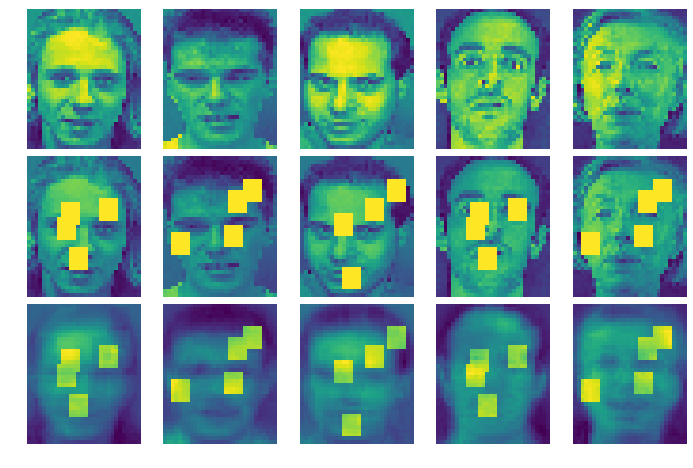
\includegraphics[width=\textwidth]{sklearn_orl_occluded_learn}
  \caption{Example images from the ORL dataset. The top image shows the original, the second row shows randomly generated occlusion, the third row shows the solution achieved by the sklearn benchmark}
  \label{fig:exampleofaces}
\end{figure}

\begin{figure}[h]
  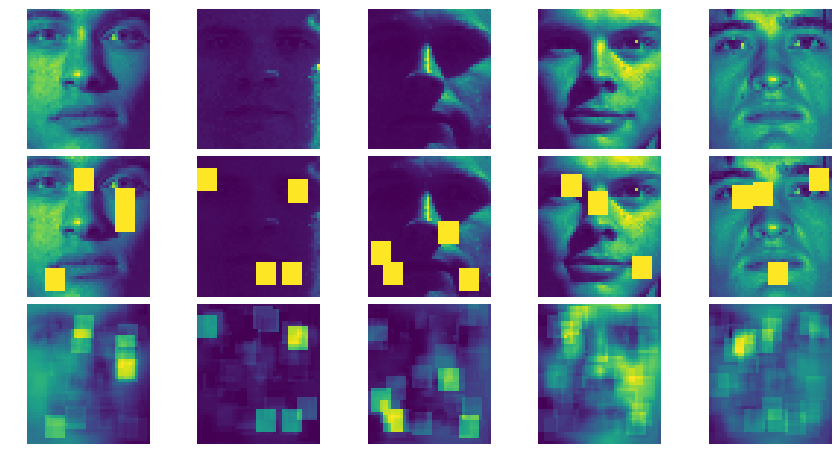
\includegraphics[width=\textwidth]{sklearn_yaleb_occluded_learn}
  \caption{Example cropped faces from the Yale dataset. The top image shows the original, the second row shows randomly generated occlusion, the third row shows the solution achieved by the sklearn benchmark}
  \label{fig:exampleyfaces}
\end{figure}


In order to measure the the performance of these different algorithms, the following metrics will be considered:\\

\subsection{Loss}
Loss is the difference between the original matrix and the reconstruction, and can be considered what information is 'lost' in the matrix factorization process. This exercise uses squared loss, given by \((Y - HW)^2\) where H and W are the dictionary and compressed representation respectively, and Y is the original image.\\

Squared loss can obscure marginal improvements later in the training process because the gains from early iterations are of a much greater magnitude. This can be rectified by using Logloss, which is given by \(ln[ (Y - HW)^2 ]\). This downweights the low-hanging fruit of early iterations and shifts the focus onto late-stage optimization.\\

\subsection{Relative Reconstruction Error}
Relative Reconstruction Error (RRE) is similar to loss, but the result is normalized by the original image. RRE is constructed by:

\[RRE = \frac{\|V - WH\|_F}{\|V\|_F}\]

where $V$ is the clean dataset, $W$ and $H$ are the dictionary and encoding respectively, and $\hat{V}$ is the noisy dataset from which $W$ and $H$ are learned.\\

\subsection{Normalized Mutual Information}

Normalized mutual information is a classification metric that can assess the ability of an algorithm at detecting the true class of some underlying data. It is given by the following equation:

\[ NMI(Y,Y_p_r_e_d) =  \frac{2 * I(Y,Y_p_r_e_d)}{H(Y) + H(Y_p_r_e_d)}\]

Normalized mutual information will be used to determine whether the reconstructed faces can capture the label information of the original data


\section{Experiment}

\subsection{Hypersurface Smoothing}

The hypersurface smoothing algorithm was designed primarily to be robust against outliers. The occlusion noise in this experiment can be considered a form of outlier, and the adjusted cost function downweights the relative importance of these pixels.

The hyperparameters were set as follows: Step size was 0.005 for both W and H matrices, rank was 10, and maximum iterations was 5000. An initial run was conducted without any occlusion, and then occlusion (n\_boxes = 3) was introduced to test for robustness. The algorithm shows rapid initial gains in decreasing loss, as shown by figure \ref{figure:hypersurface_logloss}. However, the algorithm quickly finds a ``floor'' beyond which it cannot improve further. 

\begin{figure}[h]
  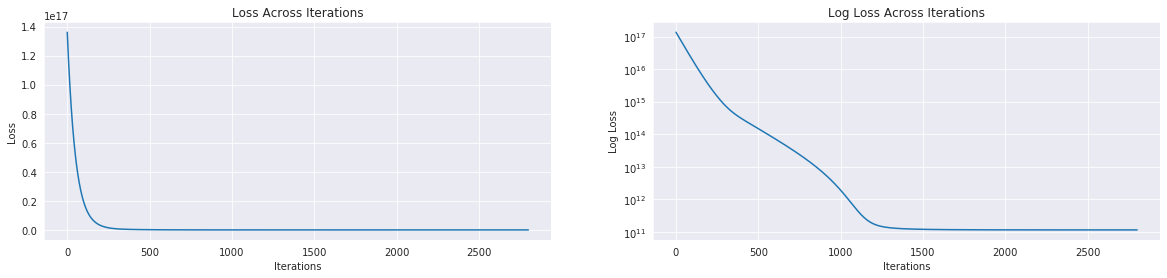
\includegraphics[width=\textwidth]{hypersurface_logloss}
  \caption{Algorithm performance as a function of training iterations. Loss declines steeply at first but levels off quickly. Log loss shows that performance improves for the initial $\frac{1}{3}$rd of the otraining process}
  \label{figure:hypersurface_logloss}
\end{figure}

The algorithm was unable to produce a sensible representation of faces from training over the cropped Yale images, as shown in \ref{figure:hypersurface_learned_faces}. However, it is possible to see some faint outlines of the facial features the algorithm is supposed to identify, such as eyes, nose and lips.  Furthermore, there are noticeable differences between faces. However, there is still substantial differences between the output and the original data, and the algorithm has also learned the occlusion in some cases.

\begin{figure}[h]
  \includegraphics[width=\textwidth]{hypersurface_learned_occlued_faces}
  \caption{The reconstruction of the data based on the hypersurface algorithm, and the training data to which the algorithm was exposed}
  \label{figure:hypersurface_learned_faces}
\end{figure}

\section{Conclusion}

\section{Reference}

\section{References}
\bibliography{report}
\bibliographystyle{apalike}
\end{document}
